\section{Spontaneous Emission I}
The most important formula we derived last class is Fermi's golden rule, which reads:
\begin{equation}
    \dod{W}{t} = \frac{2\pi}{\hbar}\abs{V_{ba}}^2\delta(E_f - E_i)\frac{d^3pd^3x}{(2\pi\hbar)^3}
\end{equation}
We consider $\frac{d^3pd^3x}{(2\pi\hbar)^3} = \dod{N}{E}dE$ and then we integrate with respect to energy to remove the delta function.

\subsection{Deriving Transitions}
Now, we want to discuss the difficult matrix element part. We have the coupling Hamiltonian:
\begin{equation}
    H = \frac{\left(\v{p} + \frac{e}{c}\v{A}\right)^2}{2m} = \frac{\v{p}^2}{2m} + \frac{e}{2mc}\left(\v{A}\cdot \v{p} + \v{p} \cdot \v{A}\right) + \mathcal{O}(\v{A}^2)
\end{equation}
We use the Coloumb gauge $\nabla \cdot \v{A} = 0$. Note this is a different gauge from what you may see in quantum field theory, where we choose Lorentz invariant Gauges. This choice of Gauge allows us to simplify:
\begin{equation}
    H = \frac{\v{p}^2}{2m} + \frac{e}{2mc}\left(2\v{p}\cdot\v{a}\right)
\end{equation}
The potential is then:
\begin{equation}
    V(\v{r}) = \frac{e}{mc}\v{p} \cdot \v{A}
\end{equation}
We have the vector potential:
\begin{equation}
    \v{A} = \v{A}_0(r)e^{-i\omega t} + \text{h.c.}
\end{equation}
where h.c. denotes the Hermitian conjugate of the first term. We consider:
\begin{equation}
    \v{A}_0 = A_0\gv{\e}e^{i\v{k} \cdot \v{r}}
\end{equation}
where $\gv{\e}$ is the polarization. We have split the plane wave into a spatial ($e^{i\v{k} \cdot \v{r}}$) and time ($e^{-i\omega t}$) piece. 

Now we will cheat\footnote{``I am an honest man, but now I am cheating'' - Ariel 2022}. In quantum mechanics, we never ever discuss the creation or annhilation of states. The number of states is fixed. Technically we need quantum field theory to discuss such transitions; but we take the semi-classical approach followed in Goswami.

We also consider the EM Hamiltonian:
\begin{equation}
    H_{EM} = \frac{1}{8\pi}\left(\v{E}^2 + \v{B}^2\right)
\end{equation}
where we have written the above in Gaussian units (in SI, the terms would be $\frac{\e_0}{2}\v{E}^2 + \frac{1}{2\mu_0}\v{B}^2$). This has the benefit of placing the electric and magnetic fields on equal footing (same energy). We therefore compute the electric and magnetic fields in our Gauge:
\begin{equation}
    \v{E} = -\frac{1}{c}\dpd{\v{A}}{t} = \frac{i\omega}{c}A_0\gv{\e}e^{-i(\omega t - \v{k} \cdot \v{r})} + \text{h.c.}
\end{equation}
\begin{equation}
    \v{B} = \nabla \times \v{A} = i(\v{k} \times \gv{\e})A_0e^{-i(\omega t - \v{k} \cdot \v{r})} + \text{h.c.}
\end{equation}

Now the cheating enters. We say that:
\begin{equation}
    \int H_{EM}d^3x = \hbar \omega
\end{equation}
everything is classical on the LHS, but the RHS is quantum. Our normalization is that the plane wave in the entire volume is normalized to a single photon with frequency $\omega$. The proper way to do it (in quantum field theory) is to quantize the electric field, but we shortcut. Computing the integral:
\begin{equation}
    \int H_{EM}d^3x = \frac{2}{8\pi}\left(\frac{\omega^2}{c^2}\abs{A_0}^2 + \left(\v{k} \times \gv{\e}_0\right)^* \cdot \left(\v{k} \times \gv{\e}_0\right)\abs{A_0}^2\right) d^3x
\end{equation}
We compute the dot product as:
\begin{equation}
    \left(\v{k} \times \gv{\e}_0\right)^* \cdot \left(\v{k} \times \gv{\e}_0\right) = \v{k}^2\abs{\gv{\e}}^2 - (\v{k} \cdot \gv{\e})(\text{h.c.})^*
\end{equation}
Now note that $\v{k} \cdot \gv{\e} = 0$ as $\v{k} \cdot \v{A} \sim \nabla \cdot \v{A} = 0$. And so:
\begin{equation}
    \left(\v{k} \times \gv{\e}_0\right)^* \cdot \left(\v{k} \times \gv{\e}_0\right) = \left(\frac{\omega}{c}\right)^2
\end{equation} 
so the integral becomes:
\begin{equation}
    \int H_{EM}d^3x = \frac{2}{8\pi}B\abs{A_0}^2\left(\frac{\omega^2}{c^2}\right)2 = \frac{V\abs{A_0}^2}{2\pi c^2}\omega^2 = \hbar\omega
\end{equation}
We therefore conclude:
\begin{equation}
    \boxed{\abs{A_0}^2 = \frac{2\pi c^2 \hbar}{\omega V}}
\end{equation}
Now let's look at the coupling part of the problem:
\begin{equation}
    V(r) = \frac{e}{mc}\v{p} \cdot \v{A} = \frac{e}{mc}\sqrt{\frac{2\pi c^2\hbar}{\omega V}}\gv{\e}e^{-i\v{k \cdot \v{r}}} \cdot \v{p}
\end{equation}
We now compute the matrix elements:
\begin{equation}
    \bra{\psi_a}\gv{\e} \cdot \v{p}e^{-i\v{k}\cdot \v{r}}\ket{\psi_b}\left(\frac{e}{mc}\right)\sqrt{\frac{2\pi\hbar c^2}{\omega V}}
\end{equation}
We then consider that:
\begin{equation}
    \abs{V_{ab}}^2\frac{d^3p d^3x}{(2\pi\hbar)^3} \to \dod{N}{E}dE \abs{V_{ab}}^2 \sim \frac{V}{V}
\end{equation}
so we see that the volume drops out! After this we can just ignore the volume entirely, now we have seen how it precisely drops out.

We already discussed how $\gv{\e} \cdot \v{k} = 0$. Suppose $\v{k} = \frac{\omega}{c}(0, 0, \zhat)$. We have multiple options for polarizations. We have $\gv{\e}^x = (1, 0, 0), \gv{\e}^y = (0, 1, 0)$, and we can also take linear combinations, e.g. the circular polarizations $\gv{\e}^+ = \frac{1}{\sqrt{2}}(1, i, 0)$, $\gv{\e}^- = \frac{1}{\sqrt{2}}(1, -i, 0)$. We call $\gv{\e}^+$ right handed and $\gv{\e}^-$ left handed. In particle physics/condensed matter, we say that it is right or left handed from the perspective of the detector. To see this:
\begin{equation}
    \v{E} = (\xhat + i\yhat)e^{-i(\omega t + ikz)} + \text{h.c.} \sim \xhat\cos(\omega t - kz) + \yhat\sin(\omega t - kz)
\end{equation}
and one can see that the wave rotates to the right, following the peak.

\begin{figure}[htbp]
    \centering
    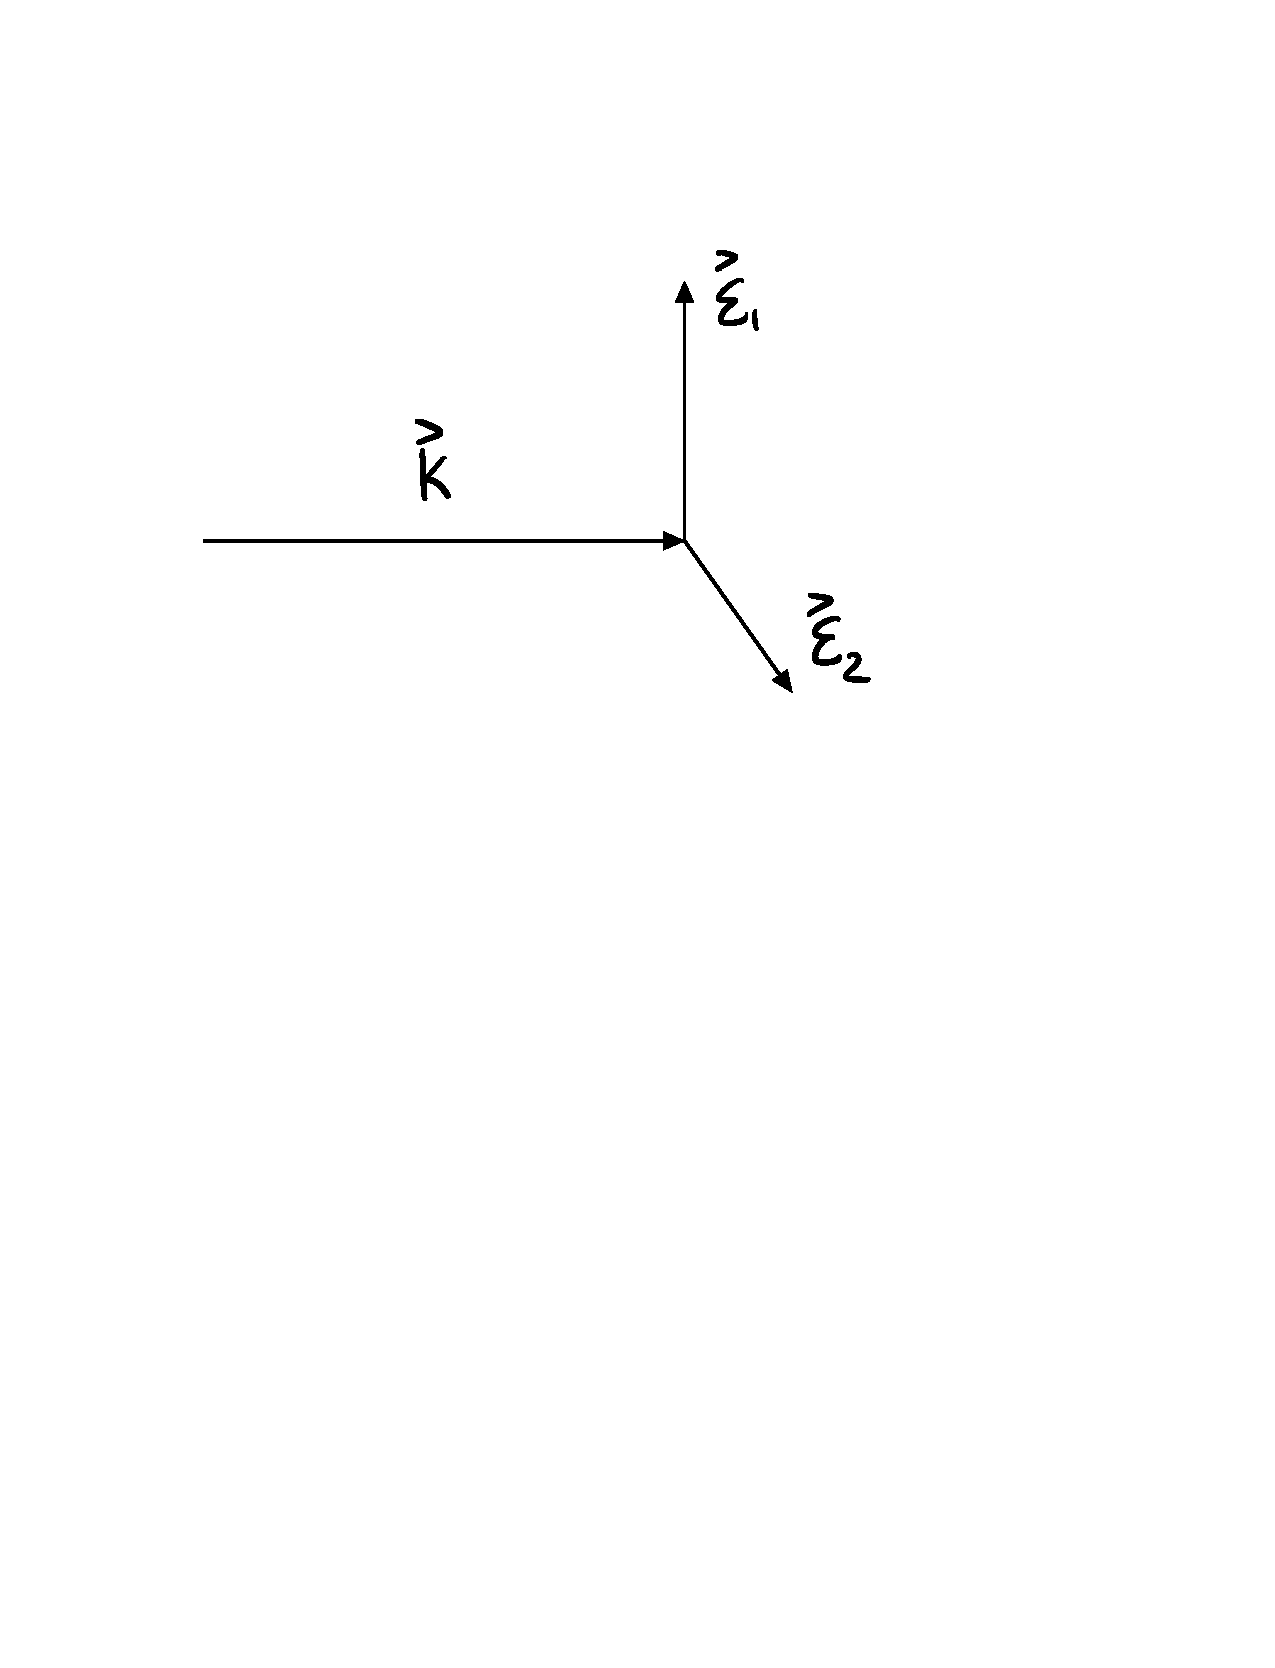
\includegraphics[scale=0.6]{Images/fig-photonpolarizations.pdf}
    \caption{We have two polarization vectors $\gv{\e}_1, \gv{\e}_2$ that are perpendicular to the direction of propogation $\v{k}$. We may take superpositions of these to construct (e.g.) circular polarized light.}
    \label{fig-photonpolarizations}
\end{figure}

Let us write down the formula with everything discussed:
\begin{equation}
    \dod{W}{t} = \int \sum_\lambda \left(\frac{2\pi}{\hbar}\right)\left(\frac{e}{mc}\right)\left(\sqrt{\frac{2\pi\hbar c^2}{\omega V}}\right)^2 \left|\bra{f}e^{-i\v{k} \cdot \v{r}}\gv{\e} \cdot \v{p}\ket{i}\right|^2\delta(E_+ - E_-)\frac{d^3pV}{(2\pi\hbar)^3}
\end{equation}
where $\sum_\lambda$ is the sum over polarizations. We will cheat one more time and borrow something from QFT. We expand in a sum over modes:
\begin{equation}
    \v{A} = \sum_{\lambda, \v{k}}\sqrt{\frac{2\pi\hbar c^2}{\omega V}}\left[\gv{\e}_\v{k}^\lambda e^{-i(\omega t - \v{k} \cdot \v{r})}a_{\v{k}, \lambda} + \gv{\e}^{*\lambda}_\v{k}e^{i(\omega t - \v{k} \cdot \v{r})}a^\dag_{\v{k}, \lambda}\right]
\end{equation}
where we have replaced the coefficients (numbers) $a_\v{k, \lambda}/a^*_\v{k, \lambda}$ with operators $a_\v{k}/a^\dag_\v{k}$ which annihilate/create photons respectively. In the diagonal form we may write:
\begin{equation}
    H = \sum_{\v{k}}\hbar\omega \left(a^\dag_{\v{k}}a_\v{k} + \frac{1}{2}\right)
\end{equation}
(there are deep hidden things here... e.g. the above energy is infinite because of the $+\frac{1}{2}$ - this puzzled physicists indeed. Related to things like Caismir effect).

We therefore consider the creation of a single photon to consider $\bra{\gamma}a^\dag_{\v{k}, \lambda}\ket{0} = 1$. What remains is to evaluate $\left|\bra{f}e^{-i\v{k} \cdot \v{r}}\gv{\e} \cdot \v{p}\ket{i}\right|^2 = 1$. 

$ka_b \sim 10^{-3}$, then $ka_B \sim \frac{\hbar\omega}{me^2c} = \frac{e^2}{\hbar c} = \alpha$ where we take $\hbar\omega$ to be a Rydberg. Why we use perturbation theory in $\alpha$ is because it is small. We will do a multiple expansion in $\alpha$ to determine transitions. We will do this next way and formulate selection rules.